\documentclass[10pt]{article}
\usepackage[margin=0.82in]{geometry}
\usepackage{amsmath,amssymb,mathtools}
\usepackage{booktabs}
\usepackage{graphicx}
\usepackage{microtype}
\usepackage{enumitem}
\usepackage{array}
\usepackage{tabularx}
\usepackage{float}
\usepackage[hidelinks]{hyperref}
\usepackage{xcolor}
\setlist{nosep}
\newcommand{\dF}{d_{\mathcal F}}
\newcommand{\Aabs}{\mathbb A}
\newcommand{\WMProfile}{\mathrm{WMProfile}}
\newcommand{\NA}{\texttt{N/A}}
\title{\textbf{Beyond ``Has a World Model?'':}\\
A Layered Profile of Predictive Abstraction, Intervention,\\
Decision Sufficiency, and Robustness under Shift\\[0.35em]
\large Post-v0.6 Research Draft with Toy C v0.1--v0.4 Extensions}
\author{Guillaume Harbonnier\\MMALS Research Program}
\date{17 September 2026}

\begin{document}
\maketitle

\begin{abstract}
The term \emph{world model} is used for systems that differ substantially in what they represent, what they predict, how they are queried, and what kinds of decisions or shifts they support. This makes the binary question ``does system $X$ have a world model?'' too coarse for technical comparison. We propose instead a declared, layered evaluation profile. L0 measures predictive closure at a stated abstraction frontier; $L1_{\rm int}$ concerns interventional validity of the abstract dynamics; L2 separates class-level decision adequacy from operational model--search adequacy; and L3 records system-level robustness under a declared shift class. Acquisition-policy exposure is not treated as an independent layer: an elementary convexity argument bounds it by L0 aliasing, so we report it only as an attribution ratio inside L0. The profile is explicitly grounded in classical state abstraction and bisimulation, approximate information states, value equivalence, self-predictive representations, causal abstraction, and recent analyses of learned planning models. Two exact finite constructions establish only that L0 and L2 are non-identical coordinates: one representation is predictively closed at a coarse abstraction while incurring positive contingent-decision regret, while a second model is exactly value-equivalent on a declared value class despite failing full-state predictive closure. We additionally give illustrative diagnostics for the geometry dependence of the acquisition-policy attribution ratio and for a minimal operational-vs-global adequacy failure. A post-v0.6 extension, Toy C, probes a different boundary: whether exact state sufficiency is distinct from possession of a future-generating model mechanism. Toy C v0.1 separates an oracle-supplied exact belief from owned predictive dynamics; Toy C v0.2 constructs a non-injective one-dimensional predictive quotient that is exact for a declared task-query family while provably insufficient for a richer nuisance query, and adds a direct-history predictor that challenges persistent recursive state storage as a necessary implementation condition. Toy C v0.3 then separates local model possession from delegated model access and finite compilation: all three can be exactly answer-equivalent on a declared finite query domain, while source removal and query-domain extension expose different capability provenance and coverage. Toy C v0.4 attacks the remaining scalar reading of extension itself: a task-specific factorised query program extrapolates exactly to longer future action horizons while failing newly conditioned-history support and hypothetical-evidence assimilation, showing that extension must be declared by axis rather than as a single modelhood discriminator. We do not claim a unique definition of world models, a necessary-and-sufficient theory, or superiority over the eliminativist alternative of reporting the underlying technical tuple directly.
\end{abstract}

\paragraph{Scope and evidence.}
The profile proposed here is an evaluation framework, not a peer-reviewed theory or a claim to a unique definition of world models. Its two main finite separation results are exact and reproducible from explicit finite environments. Other coordinates combine literature-grounded criteria with evaluation contracts that remain only partly instantiated in this manuscript, and the additional diagnostics are illustrative rather than general empirical validation. Whether the profile improves practical comparison or failure localisation beyond direct reporting of its primitive objects remains open.

\section{Introduction}

Consider two systems that can both reasonably attract the label ``world model'' while supporting very different claims. A passive, non-action-conditioned video predictor may forecast future observations accurately and therefore be predictively strong at the observation level, yet provide no declared semantics for intervention or decision. MuZero sits almost at the opposite end: its learned dynamics need not be a faithful simulator across unseen policies, yet they can support strong planning on the query distribution induced by search~\cite{schrittwieser2020,he2024}. These systems are not simply better and worse points on one scale. They answer different technical questions.

That tension recurs across the literature. Ha and Schmidhuber used the term for a learned compressed spatiotemporal model supporting policies trained inside imagined rollouts~\cite{ha2018}. PlaNet learned latent dynamics from pixels and planned in latent space~\cite{hafner2019}; Dreamer learned behaviour by latent imagination~\cite{hafner2020}. LeCun's autonomous-machine proposal places a configurable predictive world model inside a larger agent and emphasises multiple abstraction levels and joint-embedding prediction~\cite{lecun2022}. Chen et al. explicitly note the lack of consensus and propose a resource-relative, compression-oriented account~\cite{chen2026}.

The motivating question for this paper came from a narrower problem in adaptive learning: \emph{which distinctions in an agent's history may be safely discarded, and which must be preserved because later actions, evidence or tasks may make them relevant?} The label ``world model'' turned that question into several questions at once:
\begin{enumerate}
    \item What aspects of past observations are represented internally?
    \item Can the representation be advanced through an internal transition operator without reconstructing the next observation?
    \item Is the representation or model adequate for a particular planning or decision problem?
    \item Does the whole system remain adequate when the intervention regime or environment changes?
\end{enumerate}
A single yes/no predicate tends to collapse these questions. A representation can be predictively closed at one abstraction and inadequate for a decision that depends on information it discards. Conversely, a model can preserve every Bellman computation relevant to a restricted decision class while being predictively wrong about variables that the decision class ignores.

This paper therefore asks a narrower question than ``what is the true definition of a world model?'':
\begin{quote}
Can a declared profile separate technically distinct claims that are often compressed into the phrase ``has a world model'', while remaining explicit about its own limits and about existing state-abstraction theory?
\end{quote}

Our answer is a profile
\[
\WMProfile_{\mathcal D}(X)
=
\langle L0[\rho_{\rm pol}],L1_{\rm int},L2.G,L2.O,L3\rangle,
\]
where each entry is reported as \emph{pass with measured budget}, \emph{fail}, \emph{not declared}, or \emph{not applicable}. The profile is not a hierarchy: the coordinates quantify different questions, and the finite evidence in this paper establishes only non-identity of L0 and L2 in two controlled constructions.

The main contributions are deliberately modest:
\begin{itemize}
    \item We formulate L0 as a \emph{predictive abstraction frontier}: the report names the finest tested abstraction level at which declared budgets hold and, when available, a natural richer level that fails.
    \item We separate class-level decision adequacy (L2.G) from operational model--search adequacy (L2.O), so that performance measured on a planner's self-induced query distribution is not silently read as a global claim.
    \item We show exactly in finite constructions that $L0\not\Rightarrow L2$ and $L2.G\not\Rightarrow L0$ under explicit declarations. Interventional validity remains a separate coordinate, while acquisition-policy exposure is retained only as an attribution diagnostic inside L0.
    \item In a post-v0.6 falsification cycle, Toy C separates current-state sufficiency from future-query capability, tests a genuinely information-losing predictive quotient and a direct-history sequence predictor, distinguishes local model possession from delegated access and finite compiled answers, and finally shows that extension/generalisation must itself be typed by axis before any new framework layer is considered.
\end{itemize}

We keep a competing eliminativist position alive throughout: the term \emph{world model} may ultimately add less than a direct report of $(\sigma,K,\text{sufficiency class},\text{shift class},\ldots)$. The paper's burden is therefore not to defend a label, but to show whether the profile improves localisation of what a system has and has not demonstrated.

\section{Lineage and related work}

\subsection{Internal models, regulation, and anticipation}

The intuition that intelligent regulation requires an internal surrogate of external dynamics predates modern machine learning. Craik argued that nervous systems can carry internal models that parallel external events and allow anticipation~\cite{craik1943}. Conant and Ashby formalised a closely related regulator-model relation under explicit assumptions in the good-regulator theorem~\cite{conant1970}. We cite these works as conceptual lineage only; the present profile is not a derivation of either theorem.

Modern world-model systems made the idea computational. Ha and Schmidhuber combined compressed visual representations with recurrent dynamics~\cite{ha2018}. PlaNet explicitly learned a transition model, observation model, reward model, and approximate belief from history, then used the latent dynamics for planning~\cite{hafner2019}. Dreamer shifted behaviour learning into imagined latent trajectories~\cite{hafner2020}. MuZero demonstrated that a learned model need not reconstruct environment observations or rules to support high-performance planning; it can instead preserve reward, value and policy-relevant predictions~\cite{schrittwieser2020}. These systems motivate the question of what a model must preserve, but they do not by themselves define a universal criterion.

\subsection{Abstraction is not new}

Any framework that compresses histories into latent states must be positioned against classical abstraction theory. Givan, Dean and Greig developed stochastic bisimulation and model minimisation~\cite{givan2003}. Ferns, Panangaden and Precup introduced bisimulation metrics and value-related bounds~\cite{ferns2004}. Li, Walsh and Littman organised state abstractions ranging from model-irrelevance to value-, action-, and policy-oriented notions~\cite{li2006}. The present L0 coordinate is therefore not proposed as a new theory of state abstraction. Its closest analogue is a reward-free/model-level abstraction claim, augmented here by an explicit query-defined frontier and embedded in a profile that separately records decision and robustness claims.

This distinction matters because the profile's contribution, if any, cannot be ``abstraction exists''. State abstraction, approximate information states and value-equivalent modelling already provide mature formalisms for different parts of the problem. They are often reported under different technical contracts, however, so evidence established in one register can be read as evidence in another. The proposed contribution is therefore a reporting and localisation discipline: declare which abstraction is being preserved, which decision class is being protected, and which robustness or intervention claim is actually being made.

\subsection{Information states and decision-relative adequacy}

In partially observed systems, the full observation-action history can be replaced by an information state when that statistic is sufficient for the relevant dynamic program. Approximate Information State (AIS) makes this operational by defining reward- and next-information-state approximation conditions under a declared integral probability metric and deriving value/policy-loss guarantees under the theorem assumptions~\cite{subramanian2022}. This addresses a central weakness of vague phrases such as ``sufficient representation'': it provides checkable conditions that imply decision guarantees.

Value Equivalence (VE) approaches adequacy from a different direction. Instead of asking whether a history statistic approximates an information state, it asks whether a learned model induces the Bellman computations that matter over declared policy and value-function classes~\cite{grimm2020}. Proper and approximate variants extend the programme~\cite{grimm2021,grimm2022}. These literatures motivate our decision-relative L2 coordinate. They also prevent us from claiming as novel the generic fact that preserving one-step or restricted predictive quantities is weaker than preserving all longer-horizon decision structure.

\subsection{Self-predictive representations and abstraction level}

Self-predictive reinforcement-learning work analyses representations that can predict their own next latent state and relates such conditions to other state/history abstractions~\cite{ni2024}. LeCun's JEPA-oriented proposal similarly emphasises prediction in representation space and multiple abstraction levels rather than reconstruction of all observation details~\cite{lecun2022}. These ideas motivate two commitments in L0: the model must support internal predictive closure, and the abstraction level must be declared rather than left implicit.

This is also why a video generator is not excluded by definition. If the declared abstraction level is the observation itself, an accurate video generator may pass L0 there. That says nothing about whether the same system passes at a causal, object-centric, control-relevant, or decision-relevant abstraction.

\subsection{Planning, query distributions, and extractable models}

A planner and a learned model cannot always be separated cleanly by interface. He et al. show that MuZero's learned model generalises poorly to evaluating unseen policies, while the policy prior in search steers computation towards regions in which the model is more accurate~\cite{he2024}. This motivates our separation between class-level adequacy and operational model--search adequacy.

Complementary capability theorems show that sufficiently general goal-directed agents contain enough predictive information for an environment model to be extracted from their policies~\cite{richens2025}. Cifuentes extends this type of result to stochastic agents under partial observability~\cite{cifuentes2026}. These theorems defeat simple interface-based exclusion rules: a system need not expose a module called ``world model'' for predictive environment structure to be recoverable from its behaviour. They do not, however, establish that a planner component is identical to a world model.

\subsection{Causal abstraction and robustness under shift}

Intervention on a lossy quotient is not automatically well defined. Work on causal abstraction and exact transformations formalises when causal relationships survive abstraction~\cite{rubenstein2017,beckers2019}. Richens and Everitt further show, under their stated robustness conditions involving local interventions on all environment variables, that robust agents must encode extractable approximate causal structure~\cite{richens2024}. We therefore keep causal/interventional validity separate from ordinary predictive closure and make robustness claims relative to a declared shift class rather than treating causality as constitutive of every world model.

\subsection{Definition by resources versus definition by task}

Chen et al. propose a recent perspective in which world models are fundamentally compression-based models of world transition processes under finite computational resources~\cite{chen2026}. That view is importantly different from task-relative definitions that make decision usefulness constitutive. Our profile separates these concerns: L0 is task-free but abstraction-relative; task-relative sufficiency enters only at L2. This does not make the profile compatible with every definition. It is better understood as an explication syntax for reporting what a system demonstrably preserves.

\section{A declared world-model profile}

Let the history at time $t$ be
\[
h_t=(o_{\le t},a_{<t})\in\mathcal H,
\]
and let a representation map compress history to
\[
z_t=\sigma(h_t)\in\mathcal Z.
\]
Let $a_t\in\mathcal A$, and let $d_{\mathcal F}$ denote a declared integral probability metric (IPM).

Before reporting any layer, declare
\[
\mathcal D=
\Big(
\underbrace{\Aabs,H_{\Aabs},\Omega_0,\mathcal F,\mathcal B}_{L0};
\underbrace{\mathcal I}_{L1_{\rm int}};
\underbrace{\mathcal T,H,\Pi,\pi_{\rm ref},\mathcal U,\varepsilon,R,\mathcal N}_{L2};
\underbrace{\Delta,\pi_{\rm ref}}_{L3}
\Big).
\]
Here $\Aabs$ is a family of measurable queries $q:S\to Y_q$ that defines the abstraction level; $H_{\Aabs}$ is a rollout horizon; $\Omega_0$ the support over which the claim is made; $\mathcal B$ a behaviour/acquisition-policy class; $\mathcal I$ a family of interventions; $(\mathcal T,H,\Pi,\pi_{\rm ref},\mathcal U,\varepsilon,R)$ a decision contract; $\mathcal N$ an off-prior evaluation family or equivalent coverage condition; and $\Delta$ a shift class.

An undeclared component has no default. A layer is reported as \emph{pass with measured budget}, \emph{fail}, \emph{not declared}, or \emph{not applicable}. The reporting discipline is structurally similar to engineering qualification: scope is fixed before measurement, budgets and admissible-case coverage are explicit, and an untested condition is not reported as a pass.

\begin{table}[t]
\centering
\caption{Interpretation of the profile coordinates. Acquisition-policy exposure $\rho_{\rm pol}$ is an L0 diagnostic, not an independent layer.}
\begin{tabularx}{\linewidth}{@{}lX X@{}}
\toprule
Coordinate & Question & Typical evidence \\
\midrule
L0 & What predictive abstraction is closed and retained? & Aliasing, fit, rollout, query-retention frontier \\
$\rho_{\rm pol}$ & How much of an existing L0 aliasing defect can the declared acquisition-policy class expose? & Mixture-diameter attribution ratio \\
$L1_{\rm int}$ & Are abstract transition claims interventionally valid? & Causal-abstraction guard, interventional calibration \\
L2.G & Is the model/representation adequate over the declared decision class? & AIS or VE-style criteria; direct regret \\
L2.O & Is the actual model--search pair adequate where it queries, and how fragile is that claim off-prior? & In-prior error + off-prior family/coverage \\
L3 & Is the whole system robust under a declared shift class? & Uniform regret or task-specific robustness criteria \\
\bottomrule
\end{tabularx}
\end{table}

\subsection{L0: predictive closure at an abstraction frontier}

The operational question is not whether a latent model is ``predictive'' in the abstract, but whether histories that the representation treats as equivalent remain interchangeable under the projected dynamics and whether the declared properties of interest survive that quotient.

Define the true projected one-step law
\[
P_\sigma(\cdot\mid h,a)
=
\mathrm{Law}\!\left(\sigma(H_{t+1})\mid H_t=h,A_t=a\right)
\]
and a candidate latent transition kernel $K(\cdot\mid z,a)$.

\paragraph{Aliasing floor and kernel fit.}
Two failures are easy to conflate. The first belongs to the compression: if $\sigma$ merges two histories, do their projected successor laws actually agree? The second belongs to the learned operator: given that compression, does $K$ reproduce those projected laws?

For histories collapsed to the same latent,
\[
\delta_{\rm alias}
=
\sup_{\substack{h,h'\in\Omega_0\\\sigma(h)=\sigma(h')}}
\sup_a
\dF\!\left(P_\sigma(\cdot\mid h,a),P_\sigma(\cdot\mid h',a)\right).
\]
The associated worst-case fit is
\[
\delta_{\rm fit}
=
\sup_{h\in\Omega_0}\sup_a
\dF\!\left(K(\cdot\mid\sigma(h),a),P_\sigma(\cdot\mid h,a)\right).
\]
For the sup/IPM form,
\[
\delta_{\rm alias}\le 2\delta_{\rm fit},
\qquad
\frac{\delta_{\rm alias}}2
\le \inf_K\delta_{\rm fit}(K)
\le \delta_{\rm alias}.
\]
We treat this as an elementary triangle-inequality consequence, not as a novelty claim. Under these worst-case definitions, the two quantities are linked: $\delta_{\rm fit}=0$ forces $\delta_{\rm alias}=0$. Their practical separation is clearest when model training reports an \emph{averaged} fit loss. A kernel can fit the average next-latent law in a cell while the histories inside that cell disagree strongly. $\delta_{\rm alias}$ then identifies disagreement caused by the quotient itself rather than by insufficient optimisation.

There is an equally important limitation. $P_\sigma$ and $K$ are compared after projection through $\sigma$ on both sides. A distinction erased by $\sigma$ is absent from both laws and can therefore be invisible to $\delta_{\rm alias}$, $\delta_{\rm fit}$ and $\delta_{\rm roll}$. These quantities measure internal coherence of the projected dynamics, not the external adequacy of what was retained. The query-retention term below supplies that external reference.

\paragraph{Conditional rollout closure.}
For legal action sequence $a_{t:t+k-1}$,
\[
\delta_{\rm roll}(k)
=
\sup
\dF\!\left(
K^k(\cdot\mid\sigma(h),a_{t:t+k-1}),
P_\sigma^k(\cdot\mid h,a_{t:t+k-1})
\right).
\]
The word \emph{conditional} is load-bearing. A model could ignore its starting state yet match an unconditional long-run marginal, while being useless for the planning question ``where do I end up from here under these actions?'' Hence the comparison is conditioned on the starting history and action sequence. Each horizon-indexed report also carries an admissible case count: termination can remove every relevant continuation at a later horizon, and an empty case set is \NA, not a zero-error success.

\paragraph{Query retention and external reference.}
For each declared query $q\in\Aabs$,
\[
\eta_q(k)
=
\inf_{g_q}\sup
 d_q\!\left(
\mathrm{Law}(g_q(\hat Z_{t+k})),
\mathrm{Law}(q(S_{t+k})\mid h,a_{t:t+k-1})
\right),
\qquad 0\le k\le H_{\Aabs}.
\]
Unlike the projected-dynamics quantities, $\eta_q$ is anchored to something the model did not generate: the declared external query $q(S)$. The price is labelled, oracle, or otherwise justified access to that reference. The $k=0$ term is essential because reproducing a future distribution is weaker than decoding the property now. A representation may forecast the correct marginal of a query while having erased which value is currently true.

Toy A below exposes both issues. At the phase abstraction the projected process is exact. When the mode query is added, $\eta_{q_{\rm mode}}(0)=\eta_{q_{\rm mode}}(1)=1$ under the L1-TV convention. At $k=2$ the raw error becomes zero only because the mode-bearing revealed histories have terminated; the report therefore includes query-bearing case counts and marks that horizon as non-informative rather than as recovered decodability.

\paragraph{The abstraction frontier.}
An L0 statement is therefore not simply ``the system passes L0''. It reports
\[
\Aabs^*=\text{finest tested abstraction level at which the declared budgets pass},
\]
paired, where possible, with a natural richer level that fails. For a frontier-style claim, a pass without a tested richer level or another non-vacuity certificate is incomplete: it shows that the chosen $\Aabs$ was easy enough, but not where the representation stops being adequate. Toy A's useful statement is thus ``phase passes; phase+mode fails; the separating query is the one later required by the decision'', not merely ``L0 passes''.

\subsection{Policy exposure as an L0 attribution diagnostic}

A change of acquisition policy can alter which full histories are mixed inside one latent cell. It cannot create a compression defect that the cell does not already contain.

For behaviour policy $\beta$, define
\[
K_\beta^\sigma(\cdot\mid z,a)
=
\int P_\sigma(\cdot\mid h,a)\,dP_\beta(h\mid z,a).
\]
The behaviour-induced discrepancy is evaluated only where both behaviour policies support the same latent--action pair:
\[
\delta_{\rm inv}^{\rm latent}
=
\sup_{\beta,\beta'\in\mathcal B}
\sup_{(z,a)\in \mathrm{supp}_\beta(Z_t,A_t)\cap\mathrm{supp}_{\beta'}(Z_t,A_t)}
\dF\!\left(
K_\beta^\sigma(\cdot\mid z,a),
K_{\beta'}^\sigma(\cdot\mid z,a)
\right).
\]
Without this common-support condition, one of the two conditional kernels may be undefined at the point being compared. Let $w^\beta$ and $w^{\beta'}$ denote the corresponding mixture weights over the member histories of a fixed latent cell. An elementary mixture-diameter argument gives
\[
\dF\!\left(K_\beta^\sigma,K_{\beta'}^\sigma\right)
\le
\frac12\lVert w^\beta-w^{\beta'}\rVert_1\,\delta_{\rm alias}
\le \delta_{\rm alias}.
\]
Consequently
\[
0\le \delta_{\rm inv}^{\rm latent}\le\delta_{\rm alias}.
\]
We make no novelty claim for this mixture bound; a dedicated prior-statement search remains a manuscript obligation.

When $\delta_{\rm alias}>0$ and the behaviour class $\mathcal B$ is explicitly restricted, we report
\[
\rho_{\rm pol}
=
\frac{\delta_{\rm inv}^{\rm latent}}{\delta_{\rm alias}}
\in[0,1].
\]
The interpretation is attribution, not another world-model axis: how much of an existing quotient defect can the declared acquisition class expose? A behaviour change that cannot place weight on the histories carrying the defect leaves it unobserved, not absent. A latent cell with only two member histories reduces $\rho_{\rm pol}$ to behaviour-weight spread; Sec.~\ref{sec:rho3} shows why cell geometry matters once three member laws are present.

\subsection{$L1_{\rm int}$: interventional validity}

Action conditioning records what happened when an action was \emph{chosen}; an interventional claim concerns what would happen if that action were \emph{set}. If the mechanism choosing the action has access to information not represented in the conditioning variables, the two laws can differ because of confounding rather than transition-model error.

We therefore assert an abstract interventional quantity only when $\sigma$ is compatible with a declared causal abstraction or exact-transformation relation for intervention family $\mathcal I$~\cite{rubenstein2017,beckers2019}. When well posed,
\[
\delta_{\rm do}
=
\sup_{z,a}
\dF\!\left(
K(\cdot\mid z,a),
\mathrm{Law}(\sigma(H_{t+1})\mid z_t=z,\mathrm{do}(A_t=a))
\right).
\]
In an unconfounded online setting in which the agent action is the sole intervention point, the interventional law can coincide with ordinary action-conditioned transition fit. In that case the report should state that $L1_{\rm int}$ adds no independent information in the declared setting; \emph{not applicable} is reserved for cases in which the intervention question itself is outside scope. Additional empirical content arises with confounded offline data or interventions on variables beyond the agent action. This draft does not yet claim a dedicated empirical $L1_{\rm int}$ separation.

\subsection{L2: global and operational decision adequacy}

L2 is explicitly task-relative. Two established routes are useful but answer different questions. AIS asks whether a compressed history statistic approximately preserves reward and next-information-state predictions well enough to support approximate dynamic programming~\cite{subramanian2022}. VE instead asks whether the model preserves Bellman computations over declared policies and value functions~\cite{grimm2020,grimm2021,grimm2022}. We keep both because they quantify different objects.

We further separate:
\begin{itemize}
    \item \textbf{L2.G}: adequacy over the declared class $(\mathcal T,H,\Pi,\pi_{\rm ref},\ldots)$;
    \item \textbf{L2.O}: adequacy of the actual model--search pair under the planner-induced query distribution $\mu_\Pi$.
\end{itemize}
The distinction matters because $\mu_\Pi$ need not be exogenous. A planner steered by the model's own scores can avoid regions the model calls unpromising, including regions it calls unpromising because it is wrong there. Error measured only under $\mu_\Pi$ can therefore partly measure the system's own avoidance behaviour: the model influences where it is examined, and it is examined where it appears accurate. This is the failure mode motivating the L2.G/L2.O split~\cite{he2024}.

Operational evaluation must additionally report either
\[
E_{\rm off}^*=\sup_{\nu\in\mathcal N}E_\nu[\ell]
\]
or a declared coverage/concentrability coefficient such as
\[
C(\nu\Vert\mu_\Pi)=\sup_{z,a}\frac{\nu(z,a)}{\mu_\Pi(z,a)}.
\]
A single convenient off-prior distribution is not enough, because it is selected by the same evaluator reporting the result. Regret always names its comparator:
\[
\mathrm{Regret}(\pi;\pi_{\rm ref})=V^{\pi_{\rm ref}}-V^\pi.
\]

\subsection{L3: robustness under declared shift}

L3 is system-level:
\[
\sup_{\delta\in\Delta}
\mathrm{Regret}_\delta(\pi;\pi_{\rm ref})\le\rho.
\]
A low system-level regret does not license a claim that one latent transition kernel is robust. Online adaptation can compensate for it; memory can identify the regime; replanning can correct a poor prediction at query time; or another component can mask the internal failure. L3 therefore records a property of the system under $\Delta$, not of any one module.

Causal-robustness results such as Richens and Everitt's must also be imported with their explicit intervention scope and extractability interpretation~\cite{richens2024}. Their result concerns robustness to specified local interventions on all environment variables under theorem assumptions and extractable causal structure; it is not a blanket claim that every robust system explicitly stores a causal model.

\section{Exact finite evidence}

\subsection{Toy A: predictive closure at a coarse frontier, contingent decision failure}

Let hidden mode $M\in\{0,1\}$ be uniform. Before termination, the agent is in an unrevealed phase $u$ or a revealed phase $r$. At $u$ it may choose \texttt{commit0}, \texttt{commit1}, or \texttt{probe}. A probe costs $c$ and reveals $M$ perfectly; at $r$ the agent then commits. A correct commit yields reward 1 and an incorrect commit reward 0.

Consider the coarse representation
\[
\sigma_C(h)=\text{phase}(h),
\]
which deliberately merges the revealed histories for $M=0$ and $M=1$. The mechanism is simple: the hidden mode enters the reward but does not enter the projected phase dynamics. L0 is reward-free, so the phase quotient can be exactly closed even though it has erased the distinction that later determines which commitment is correct.

At
\[
\Aabs_{\rm phase}=\{q_{\rm phase}\},
\]
exact enumeration gives
\[
\delta_{\rm alias}=\delta_{\rm fit}=\delta_{\rm roll}(1)=\delta_{\rm roll}(2)=0,
\]
and zero phase-query error on every informative horizon. Yet at the richer
\[
\Aabs'=\{q_{\rm phase},q_{\rm mode}\},
\]
mode-query error is 1 at $k=0$ and $k=1$ under the L1-TV convention. At $k=2$ the raw mode-query error is zero only because the revealed, mode-bearing histories have terminated; the query-bearing case count is zero and the horizon is reported as non-informative rather than as recovered decodability.

The decision consequence is exact. Enumerating all 12 deterministic history-measurable policies and all 6 deterministic $\sigma_C$-measurable policies yields
\[
V^*_{\rm hist}(c)=\max(\tfrac12,1-c),
\qquad
V^*_C(c)=\tfrac12,
\]
so
\[
\mathrm{Regret}(c)=\max(0,\tfrac12-c).
\]
At $c=0.10$, the history-aware optimum is $0.90$, the best coarse-policy value is $0.50$, and regret is $0.40$.

Without the probe, both immediate commitments are worth $1/2$ and the coarse representation is optimal: discarding an unknowable distinction costs nothing. The probe is load-bearing because it makes the mode acquirable. For $c<1/2$, the regret can therefore be read as the value of the discarded information net of its acquisition cost,
\[
\mathrm{Regret}(c)=\tfrac12-c.
\]

\begin{figure}[t]
\centering
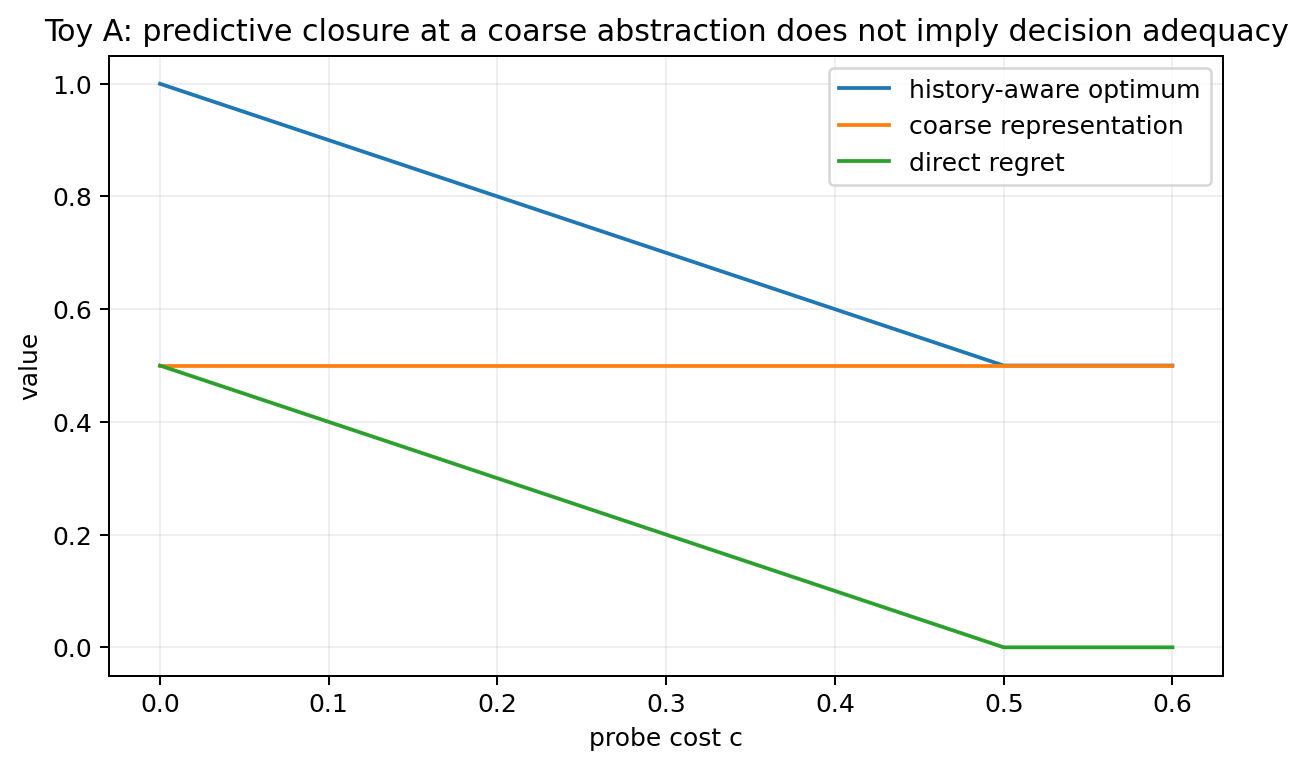
\includegraphics[width=0.79\linewidth]{fig_toy_a_regret.png}
\caption{Toy A. Predictive closure at the phase abstraction is exact, while the information-gathering action makes the discarded mode decision-relevant. Positive L2 regret is certified directly by policy enumeration.}
\label{fig:toya}
\end{figure}

This construction therefore establishes only
\[
L0(\Aabs_{\rm phase})\not\Rightarrow L2_{\rm contingent}.
\]
The certificate is direct positive regret, not failure of an AIS sufficient-condition bound. AIS AP1 error remains a diagnostic: because the hidden mode affects reward, the coarse statistic fails reward prediction at the revealed phase, but failure of a sufficient condition alone would not imply positive regret.

\subsection{Toy B: exact decision equivalence despite predictive failure}

Let state be $s=(x,n)$, where $x\in\{0,1\}$ is decision-relevant and $n\in\{0,1,2,3\}$ is nuisance noise. Actions \texttt{stay} and \texttt{flip} update $x$ deterministically. In the true model, $n'$ is uniform. An intentionally wrong model always predicts $n'=0$ while predicting the $x'$ dynamics exactly. Reward depends only on $x$.

With identity representation and full abstraction
\[
\Aabs_{\rm full}=\{q_x,q_n\},
\]
the full-state transition error is
\[
\delta_{\rm fit}=1.5
\]
under the L1-TV convention, so L0 fails for any smaller budget.

Now declare the value-function class
\[
\mathcal V_x=\{V:V(x,n)=v(x)\}.
\]
A Bellman update integrates the declared $V$ over the next-state distribution. If $V$ is constant in $n$, the $n'$ marginal disappears from that integral. Because the true and approximate models have identical $x'$ marginals and identical rewards, every Bellman update on $\mathcal V_x$ is therefore identical even though the approximate model is maximally wrong about the nuisance component. Exhaustive computation over all 256 deterministic stationary policies gives maximum Bellman gap zero.

Thus
\[
L2.G\text{-VE}=\text{pass}
\quad\text{while}\quad
L0(\Aabs_{\rm full})=\text{fail}.
\]
The limitation follows from the same mechanism: value equivalence is a property of a model paired with a declared value class. Enlarge that class to include functions sensitive to $n$, and the equivalence need not survive. This is intentionally close to classical noisy-TV/state-abstraction examples; we claim no novelty for the phenomenon itself.

\subsection{Why the two constructions form a pair}

The two directions are possible because L0 and L2 quantify over different index sets. L0 asks what a declared query family $\Aabs$ survives under the representation and its projected dynamics. L2 asks what a declared reward, policy or value-function class requires for decision. Neither declaration automatically dominates the other. The finite constructions therefore establish
\[
L0\not\Rightarrow L2,
\qquad
L2.G\not\Rightarrow L0,
\]
under explicit declarations, but they do \emph{not} establish non-collinearity in a non-degenerate regime: Toy A uses a very coarse phase abstraction, and Toy B chooses a value class blind to nuisance by construction.

\section{Post-v0.6 extension: state sufficiency versus model structure}
\label{sec:toyc}

Toy A and Toy B separate predictive and decision-relative adequacy. They do not answer a different question exposed by the POMDP belief-state comparison: if a statistic of history is already sufficient, what additional technical property, if any, turns that state into a model? Toy C attacks that question through finite counterexamples rather than by adding another profile coordinate.

\subsection{Toy C v0.1: exact current state versus future-generating capability}

Let $S_t\in\{0,1\}$, let $O_t$ be a symmetric $3/4$-accurate observation of $S_t$, and let the two actions induce identity and anti-persistent state dynamics. The exact Bayesian belief is
\[
b_t=P(S_t=1\mid h_t).
\]
The predictive state
\[
q_t=P(O_{t+1}=1\mid h_t,a_t=0)
=\frac14+\frac12 b_t
\]
can be updated and rolled forward directly in $q$-space.

Four systems are separated. Agent A receives the exact $b_t$ from an oracle at every real step but owns no transition, observation, update or rollout operator. Agent B owns the scalar predictive state and exact action-conditioned predictive/update rules but no explicit hidden-state representation. Agent C owns the full generative model and Bayesian filter. Control D memorises exact one-step predictions only on a finite training support.

Exact rational enumeration through depth four gives B/C equality on 682 representation checks, 340 one-step predictions, 680 posterior updates, 340 decision queries, 640 branch-conditioned length-three compositions and 300 open-loop action-sequence queries. The lookup control is exact on 20 memorised entries but has $0/64$ coverage on held-out depth-two queries.

This construction supports only an architectural distinction:
\[
\text{exact current epistemic state}
\;\not\equiv\;
\text{owned future-generating mechanism}.
\]
Its main limitation is deliberate: $q_t$ is an affine bijection of the complete binary belief, so v0.1 does not yet demonstrate a genuinely information-losing predictive quotient.

\subsection{Toy C v0.2: a non-injective predictive quotient}

To attack that limitation, let the hidden state be
\[
S_t=(X_t,N_t),\qquad X_t,N_t\in\{0,1\}.
\]
Action $a_t\in\{\mathrm{STAY},\mathrm{FLIP}\}$ controls only $X$: $\mathrm{STAY}$ preserves it and $\mathrm{FLIP}$ maps $X$ to $1-X$. The nuisance variable $N$ evolves independently with persistence $2/3$. Observation is the pair $O_t=(Y_t,Z_t)$ with
\[
P(Y_t=X_t)=\frac34,
\qquad
P(Z_t=N_t)=\frac45.
\]
With independent uniform priors, the full posterior factorises as $(b_t^X,b_t^N)$.

Declare a task query family involving only future $Y$ predictions and the reward $R_{t+1}=\mathbf 1\{X_{t+1}=1\}$. Agent B stores only
\[
q_t=P(Y_{t+1}=1\mid h_t,\mathrm{STAY})
=\frac14+\frac12 b_t^X.
\]
It ignores $Z$ and therefore discards the nuisance posterior $b_t^N$. Nevertheless, for the declared task family the exact action-conditioned prediction is
\[
P(Y_{t+1}=1\mid q_t,\mathrm{STAY})=q_t,
\qquad
P(Y_{t+1}=1\mid q_t,\mathrm{FLIP})=1-q_t,
\]
and the state can be updated directly after observing $Y_{t+1}$.

The verifier enumerates all reachable histories through depth three: $4,32,256,2048$ histories at depths $0,1,2,3$. All exact task-family checks pass: 2340 representation/history-recomputation checks, 584 one-step predictions, 2336 recursive updates, 584 decision checks, 2304 branch-conditioned length-two checks, and 1080 open-loop action-sequence checks.

The quotient is genuinely non-injective. Histories with the same $q_t$ can have different nuisance posteriors. Inside every $q$ cell the task-query aliasing is exactly zero,
\[
\Delta_Y=0,
\]
while the richer nuisance query has positive aliasing,
\[
\Delta_Z
=\max_{h,h':q(h)=q(h')}
\left|P(Z_{t+1}=1\mid h)-P(Z_{t+1}=1\mid h')\right|
=\frac{19}{129}.
\]
One maximal witness has the same $q=21/82$ but nuisance beliefs $17/129$ and $112/129$, which imply $P(Z_{t+1}=1)=55/129$ and $74/129$ respectively. Thus the same representation is exact for the declared task abstraction and provably insufficient for the richer query family. This is an abstraction frontier, not a global reconstruction claim.

\subsection{Agent E: falsifying a strong recursive-state requirement}

Toy C v0.2 also adds Agent E. It owns the exact task-relevant dynamics but stores no persistent recursively updated latent state. For each query it starts from the raw history, recomputes the task-relevant posterior, and evaluates the requested candidate action sequence. Formally it exposes a direct map
\[
F_E(h_t,a_{t:t+k-1})
=
P(Y_{t+k}=1\mid h_t,a_{t:t+k-1}).
\]
It matches Agents B and C on all 1080 tested open-loop action-sequence queries.

This weakens the strong hypothesis that model-like capability requires a \emph{persistently stored} recursively updateable state. Recursive state is one efficient realisation, not a necessity in this finite construction. The weaker candidate that survives is implementation-neutral: B, C and E all internally own a mechanism for answering declared future action-indexed queries away from the currently realised trajectory. Agent A does not; Control D has no such coverage off memorised support.

This is still not promoted to a definition. In particular, the construction does not establish independent causal validity, regime-shift robustness, or that the declared task family is broad enough to justify the word ``world''. It instead sharpens the next falsification target: distinguish \emph{possession} of a future-query mechanism from mere \emph{access} to model-derived answers.


\subsection{Toy C v0.3: model possession versus model access}

Toy C v0.3 attacks the strongest implementation-specific candidate left after v0.2: that a model-like system must \emph{internally own} the action-indexed future-query mechanism. The stochastic environment is unchanged. Instead, the location and form of predictive capability are varied.

Declare the finite benchmark
\[
\mathcal D_0
=
\{(h_t,a_{t:t+k-1}):t\le2,\;k\in\{1,2,3\}\},
\]
with query
\[
Q(h_t,a_{t:t+k-1})
=
P(Y_{t+k}=1\mid h_t,a_{t:t+k-1}).
\]
Exact enumeration gives $|\mathcal D_0|=4088$ queries.

Three systems are compared. Agent M owns the task-relevant dynamics inside the declared local boundary and computes the query from history. Agent F owns no local transition, observation, update or rollout mechanism; while an external exact model service O is available, F simply delegates the query to O. Agent G is a finite compiled answer object containing one exact answer for every element of $\mathcal D_0$, with no declared transition, update, composition or extrapolation rule.

On the declared finite domain all three are exactly answer-equivalent:
\[
M=\frac{4088}{4088},
\qquad
F+O=\frac{4088}{4088},
\qquad
G=\frac{4088}{4088}.
\]
Thus finite answer correctness alone cannot identify whether predictive structure is locally possessed, externally accessed, or compiled into a finite query table.

The distinction becomes observable only after changing the qualification contract. On the horizon-four extension domain $\mathcal D_+$, containing 4672 queries, M and F+O remain exact,
\[
M=\frac{4672}{4672},
\qquad
F+O=\frac{4672}{4672},
\]
whereas G has zero coverage,
\[
\mathrm{coverage}(G,\mathcal D_+)=\frac{0}{4672}.
\]
If the external service O is removed, M remains exact on $\mathcal D_0$, F has zero defined answers, and G retains only its finite compiled domain. Source removal therefore distinguishes local possession from delegated access; query extension distinguishes a finite compiled answer object from a mechanism with wider predictive access.

The construction also makes the system boundary explicit. At the local-agent boundary, F has model \emph{access} but not model \emph{possession}. At an expanded boundary containing F+O, the composite system does contain the external predictive mechanism. We therefore treat model-location claims as boundary-relative attribution claims rather than as a new framework layer.

An elementary finite-compilation observation explains why this matters. For any finite declared query set $D$ and deterministic exact map $M:D\to\mathcal Y$, the table
\[
T_M=\{(d,M(d)):d\in D\}
\]
is observationally equivalent to M on $D$. We make no novelty claim for this fact. Its methodological consequence is that finite behavioural agreement cannot by itself establish internal generative structure. Tests of mechanism possession need additional declarations such as extension, dependency removal, architectural inspection, compositional constraints, or robustness.

Toy C v0.3 therefore weakens the strong H3-like candidate that \emph{internal ownership} is necessary for system-level future-query capability. What survives is better expressed as a capability contract: which future queries can be answered, over what domain, from what source, within which declared system boundary, and with what behaviour under extension, source removal, intervention and shift.


\subsection{Toy C v0.4: typed extension without full generative closure}

Toy C v0.4 deliberately keeps the environment fixed and attacks a tempting over-reading of v0.3. In v0.3, a longer-horizon query domain separated the finite compiled table G from mechanisms M and F that could answer beyond the compiled support. That does not imply that \emph{extension capability} is a scalar discriminator of model-like structure.

Agent H is a task-specific factorised query program. For each supported conditioning history through depth 2, it stores one scalar seed
\[
q(h)=P(Y_{t+1}=1\mid h,\mathrm{STAY}).
\]
There are exactly 292 such seeds. H declares no hidden-state model, nuisance model, observation-update rule, recursively stored latent state, or external model service. It uses only the algebraic identity induced by the deterministic task dynamics: an even number of future \texttt{FLIP} actions preserves the task belief and an odd number complements it. Hence
\[
Q_H(h,a_{t:t+k-1})=
\begin{cases}
q(h), & \text{even number of FLIPs},\\
1-q(h), & \text{odd number of FLIPs}.
\end{cases}
\]
The construction intentionally does not decide whether H should be called a model.

On the baseline domain $\mathcal D_0$ from v0.3, all four mechanisms are exact:
\[
M=F+O=G=H=\frac{4088}{4088}.
\]
The compiled table G contains 4088 query-answer entries, while H uses 292 history seeds plus one rule. The ratio $4088/292=14$ is bookkeeping only; we make no compression, Kolmogorov-complexity, or MDL claim because the description length of H's rule is not included.

The first extension changes only the future action horizon. Keeping the same conditioning histories, action-sequence lengths 4, 5 and 6 produce 32704 new endpoint queries. M and F remain exact, G has no entries, and H remains exact without new per-query cache entries:
\[
M=F+O=H=\frac{32704}{32704},
\qquad
\mathrm{coverage}(G)=\frac{0}{32704}.
\]
The parity identity is additionally checked by exact rational arithmetic for all 292 supported histories and all binary action sequences of lengths 1 through 8, giving $148920/148920$ exact comparisons.

The second extension changes a different axis. Returning to action lengths 1--3 but conditioning on newly observed histories at depth 3 yields 28672 queries. M and F can reconstruct the task belief from the new history, whereas neither G nor H has a corresponding entry or update rule:
\[
M=F+O=\frac{28672}{28672},
\qquad
G=H=\frac{0}{28672}\text{ defined}.
\]
Thus future-horizon extension and conditioning-history extension are distinct capabilities in this finite construction.

A third query makes the distinction sharper by requiring assimilation of hypothetical future evidence before prediction continues:
\[
P(Y_{t+2}=1\mid h_t,a_0,Y_{t+1}=y_1,a_1).
\]
The domain contains 2336 branch-conditioned queries. M and F are exact on all of them; G and H expose no such interface. Open-loop endpoint extrapolation is therefore distinct from branch-conditioned evidence assimilation.

Source removal also ceases to be a scalar discriminator. Once the external oracle O is removed, F becomes undefined on the baseline domain, but H remains exact on both the 4088 baseline queries and the 32704 longer-horizon queries. Local availability plus source independence plus long-horizon extrapolation still does not identify a full generative/update model under the declared interface.

The methodological residue is a typed extension contract rather than a new layer:
\[
E=(E_{\rm horizon},E_{\rm history},E_{\rm query},E_{\rm branch},E_{\rm source},E_{\rm intervention},E_{\rm shift}).
\]
This tuple is exploratory metadata. Toy C v0.4 weakens the hypothesis that generic ``extension beyond the benchmark'' is a scalar modelhood discriminator. It does not establish a universal taxonomy of extension axes, causal validity, regime-shift robustness, or a necessary-and-sufficient definition of world model.

\section{Illustrative diagnostics}

The following examples illustrate two properties of the profile that are not established by the two finite non-implication constructions alone.

\subsection{A three-history witness for $\rho_{\rm pol}$}
\label{sec:rho3}

With only two member laws in a latent cell, every behaviour-induced mixture lies on the line segment joining those laws. The distance between two mixtures is then forced to scale with the behaviour-weight displacement, so the ratio $\rho_{\rm pol}$ cannot demonstrate dependence on richer cell geometry.

Consider instead three histories and the same two behaviour mixtures
\[
w=(0.5,0.5,0),
\qquad
w'=(0,0.5,0.5).
\]
Their half-L1 weight spread is $\tfrac12\lVert w-w'\rVert_1=0.5$. The mixture bound from Sec.~3 implies
\[
\rho_{\rm pol}\le \frac12\lVert w-w'\rVert_1=0.5.
\]

In geometry 1, let the projected laws be $(\delta_A,\delta_B,\delta_C)$. Then $\delta_{\rm alias}=2$, the two behaviour mixtures are at distance $1$, and
\[
\rho_{\rm pol}=0.5,
\]
so the bound is tight. In geometry 2, let the laws be
\[
\delta_A,\quad \delta_B,\quad 0.8\delta_A+0.2\delta_B.
\]
The same $\delta_{\rm alias}=2$ and the same behaviour-weight spread now produce mixture distance $0.2$ and
\[
\rho_{\rm pol}=0.1.
\]
The third law lies inside the convex hull of the first two, so a substantial weight displacement can move the induced mixture only slightly. The slack in the bound is therefore geometric: $\rho_{\rm pol}$ depends jointly on what behaviour weights are reachable and on how the member laws are arranged inside the aliased cell.

\begin{figure}[t]
\centering
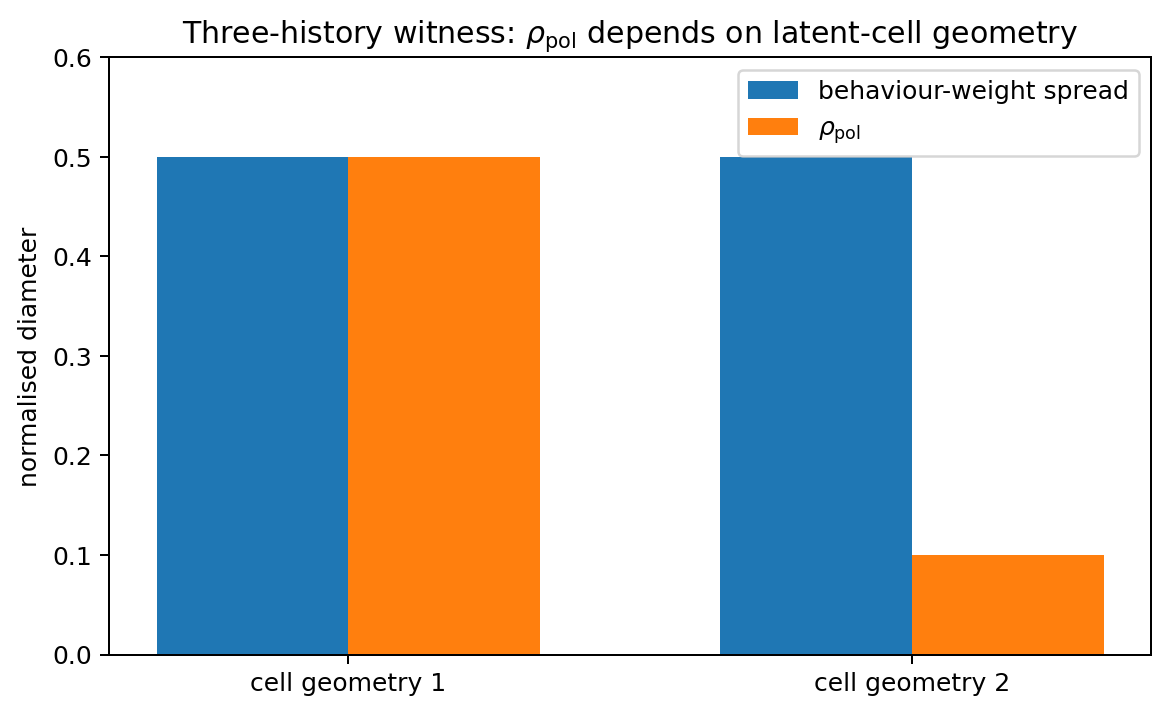
\includegraphics[width=0.66\linewidth]{fig_rho_three_history.png}
\caption{Same declared behaviour-weight spread, different $\rho_{\rm pol}$ because the latent-cell law geometry differs. This illustrates attribution; it is not a novelty claim.}
\label{fig:rho3}
\end{figure}

This construction isolates the first non-degenerate case in which $\rho_{\rm pol}$ can depend on latent-cell geometry rather than only on behaviour-weight spread. It does not elevate $\rho_{\rm pol}$ into a separate coordinate.

\subsection{A minimal L2.O witness}

L2.O exists because the model can influence the query distribution under which its own accuracy is measured. A deliberately minimal two-action example makes the loop explicit.

Suppose the true one-step returns are
\[
Q_{\rm true}(a_{\rm safe})=1,
\qquad
Q_{\rm true}(a_{\rm unseen})=2,
\]
while the learned model predicts
\[
\hat Q(a_{\rm safe})=1,
\qquad
\hat Q(a_{\rm unseen})=0.
\]
A greedy planner under the learned model therefore selects $a_{\rm safe}$ and induces
\[
\mu_\Pi(a_{\rm safe})=1.
\]
The operational prediction error is zero precisely because the model's own error on $a_{\rm unseen}$ makes the planner avoid querying it. Under a uniform off-prior evaluation distribution, however, the mean absolute error is 1, and the planner incurs regret 1 against the global optimum.

The construction is intentionally minimal; it is not a model of MuZero. It isolates the closed loop motivating L2.O: the model shapes the operating points on which it is evaluated. A representative empirical test would require a learned model and search procedure whose query distribution is genuinely endogenous, together with a declared off-prior family or non-vacuous coverage coefficient.

\section{What does the profile add beyond a flat tuple?}

The strongest criticism of the proposal is eliminativist. Every reported quantity is ultimately derived from more primitive objects such as the representation $\sigma$, the transition operator $K$, declared decision classes, resources and shift classes. Why not retire ``world model'' as a technical term and report
\[
(\sigma,K,\text{sufficiency class},\text{shift class},\text{resources},\ldots)
\]
directly? Naming a bundle of derived quantities does not create a natural kind, and the profile adds no raw information that could not in principle be represented elsewhere. This criticism remains live.

The current positive case has three parts, and they are not equally strong.

\paragraph{The abstraction frontier.}
This is the strongest profile-level object at present. A single-level tuple reports a point: one chosen $\Aabs$ and its errors. The frontier reports where that claim stops. ``Phase passes, phase+mode fails'' requires testing and recording at least two levels and naming the separating query. The informational gain is therefore not a new primitive, but an enforced comparison across declared levels.

\paragraph{Bidirectional non-implication.}
The exact toys show that predictive abstraction and decision adequacy are not two names for the same condition. This is useful defensively, but the flat tuple can represent the same fact. The finite evidence therefore establishes non-identity, not superiority of the profile.

\paragraph{L2.G versus L2.O.}
This may be the most useful distinction operationally: a model--search pair can look accurate on the distribution it induces while being poor on the larger declared class. But that distinction would remain valuable even if the phrase ``world model'' disappeared tomorrow. It is a methodological argument for how to evaluate model--search systems, not evidence that a new natural kind has been discovered. He et al.'s analysis of MuZero provides a retrospective example rather than a prediction of this framework: evaluation confined to the search-induced region would miss the model's poorer evaluation of unseen policies, whereas widening the query contract reveals the discrepancy~\cite{he2024}.

The profile earns its name only if cross-layer localisation changes what experiments we run or which failures we predict. A stronger future test would show a case where the frontier or an L2.G/L2.O distinction identifies a failure that a single-level report would have missed, or changes an ablation, shift declaration or data-collection design. Absent such evidence, the eliminativist option remains the default competitor and the burden stays on the profile.

\section{Implications for adaptive learning systems and MMALS}

The motivating scientific question behind this work is more specific than the definitional dispute. An adaptive learner cannot retain every detail of every past interaction indefinitely. It must in some sense quotient its history. The difficult question is when two histories may safely be treated as equivalent.

The profile is useful here as an instrument rather than as a label. A history compression $\sigma$ can be closed at one predictive abstraction and fail at another. It can be adequate for one decision class and fail as soon as a new information-gathering action becomes valuable. It can look accurate on the operational region induced by the current planner while being brittle outside that region. Under shift, the whole system may compensate through memory or adaptation even when one transition model is wrong.

For MMALS, the useful object is therefore not the assertion ``MMALS is a world model'', but a record of which distinctions are currently preserved, which have been deliberately quotiented away, and under which actions, evidence channels, tasks and regimes that quotient remains defensible.

The present profile still assumes that the abstraction family $\Aabs$ is declared externally. The stronger continual-learning problem is to let the abstraction itself change,
\[
\Aabs_t\rightarrow\Aabs_{t+1}.
\]
That is closer to MMALS's REUSE $\rightarrow$ ADAPT $\rightarrow$ FORK $\rightarrow$ NEW REGIME logic: preserve a quotient while it remains adequate, then refine or split it when a previously discarded distinction becomes dynamically, decisionally or causally relevant.

This yields the research question that now motivates the next stage:
\begin{quote}
Which distinctions between histories should an adaptive learner preserve, and which may it safely quotient away as its actions, evidence channels, tasks and operating regimes change?
\end{quote}

\section{Research process and transparency}

The framework evolved through an explicitly adversarial drafting process. Early versions treated ``sufficiency'' as the load-bearing constitutive word and separated model from planner too sharply. Review forced the proposal to import AIS and VE as existing decision-sufficiency frameworks, to treat interface-based boundaries cautiously, and to demote behaviour-policy invariance after it was shown to be bounded by L0 aliasing. A later executable audit found that a correct numerical result had initially been supported by a non-evidential script; the script was replaced by environment-derived enumeration and independently recomputed before the present manuscript was prepared.

This history is relevant because the final contribution is smaller than the initial proposal. We regard that reduction as evidence of process quality, not as a weakness to hide.

\paragraph{AI-assistance disclosure.}
The conceptual programme, problem selection, acceptance/rejection of claims, and final scientific responsibility belong to the author. AI systems were used extensively for literature navigation, drafting, mathematical challenge, code generation, and adversarial review. Independent review passes were themselves AI-assisted, but included checksum verification, clean reruns, independent code paths, and explicit reviewer disclosure. Any public submission should retain a concise disclosure appropriate to the venue and should not describe AI-assisted review as human peer review.

\section{Limitations}

The present evidence is intentionally narrow.

\begin{itemize}
    \item The finite constructions establish non-identity of L0 and L2 only in toy regimes.
    \item Toy A's passing abstraction is extremely coarse; it does not establish non-degenerate non-collinearity between predictive and decision adequacy.
    \item Toy B's decision class is explicitly blind to the nuisance variable.
    \item $L1_{\rm int}$ and L3 remain uninstantiated by dedicated finite witnesses in this draft.
    \item The L2.O witness is diagnostic rather than representative of learned model--search systems.
    \item The mixture-diameter inequality used to bound $\delta_{\rm inv}^{\rm latent}$ is treated as an elementary convexity property; we do not claim novelty and have not performed an exhaustive prior-statement search across probability-metric and aggregation literatures.
    \item The abstraction frontier is externally declared. Adaptive abstraction discovery and revision remain future work.
    \item Toy C v0.4 relies on a deliberately simple parity factorisation; it demonstrates axis-specific extension in this finite system, not a general factorisation theorem or formal complexity advantage.
    \item The term ``world model'' may ultimately be less useful than direct reporting of representation, dynamics, adequacy, and shift contracts.
\end{itemize}

\section{Conclusion}

The binary question ``does this system have a world model?'' often compresses several technically different claims. We proposed a smaller alternative: report predictive abstraction, interventional validity, decision adequacy, operational model--search adequacy and shift robustness separately, under an explicit declaration tuple.

The framework does not settle what a world model \emph{is}. It supplies a disciplined syntax for saying what a particular system has actually demonstrated and where that demonstration stops. Two exact finite constructions show that predictive closure and decision adequacy can come apart in both directions under declared abstractions and decision classes. A three-history diagnostic shows that policy exposure of an L0 compression defect can depend on latent-cell geometry rather than only behaviour-policy spread. A minimal L2.O example illustrates how adequacy measured only where a planner chooses to look can become self-confirming. The post-v0.6 Toy C cycle adds a different lesson: exact current-state sufficiency, task-relative predictive closure, full hidden-state reconstruction, and persistent recursive-state storage should not be silently identified. Toy C v0.2 in particular makes query breadth observable through an exact zero-versus-positive aliasing frontier and weakens a strong recursive-state necessity hypothesis before it can harden into a definition. Toy C v0.3 further shows that local possession, delegated access and finite compiled answers can be indistinguishable on a declared finite query domain, so model-location claims require an explicit system boundary and capability source. Toy C v0.4 then shows that even extension beyond that domain is not a scalar property: a small task-specific query program can extrapolate indefinitely along one declared axis while being unable to absorb one new conditioning observation or answer a branch-conditioned query.

Whether this deserves the name ``world-model profile'' remains an open explanatory question. If the profile does not improve failure localisation, comparison or experimental design, the eliminativist option should win. The more durable scientific problem is the one that motivated the exercise in the first place:
\begin{quote}
Which distinctions between histories should an adaptive learner preserve, and which may it safely quotient away as its actions, evidence channels, tasks and operating regimes change?
\end{quote}

\clearpage
\appendix
\section{Finite results summary}

\begin{table}[H]
\centering
\caption{Exact finite evidence used in the manuscript. TV values use the L1 convention $\sum_x|p(x)-q(x)|$.}
\begin{tabular}{@{}lll@{}}
\toprule
Construction & Quantity & Result \\
\midrule
Toy A & $\delta_{\rm alias},\delta_{\rm fit}$ at phase level & $0,0$ \\
Toy A & Regret at $c=0.10$ & $0.40$ \\
Toy A & Regret law & $\max(0,\frac12-c)$ \\
Toy A & $\eta_{q_{\rm mode}}(0),\eta_{q_{\rm mode}}(1)$ & $1,1$ \\
Toy B & full-state $\delta_{\rm fit}$ & $1.5$ \\
Toy B & max Bellman gap on $\mathcal V_x$ & $0$ \\
Toy C v0.1 & B/C exact open-loop checks & $300/300$ \\
Toy C v0.1 & lookup D held-out coverage & $0/64$ \\
Toy C v0.2 & task-query alias gap $\Delta_Y$ & $0$ \\
Toy C v0.2 & nuisance-query alias gap $\Delta_Z$ & $19/129$ \\
Toy C v0.2 & B/C/E exact open-loop checks & $1080/1080$ \\
Toy C v0.2 & lookup D held-out coverage & $0/512$ \\
Toy C v0.3 & M/F/G exact on declared $D_0$ & $4088/4088$ each \\
Toy C v0.3 & M/F exact on horizon-4 extension & $4672/4672$ each \\
Toy C v0.3 & compiled G horizon-4 coverage & $0/4672$ \\
Toy C v0.3 & delegated F after oracle removal & $0/4088$ defined \\
Toy C v0.4 & H exact on baseline $D_0$ & $4088/4088$ \\
Toy C v0.4 & H exact on horizon-4/5/6 extension & $32704/32704$ \\
Toy C v0.4 & H on new depth-3 conditioning histories & $0/28672$ defined \\
Toy C v0.4 & M/F branch-conditioned evidence queries & $2336/2336$ each \\
Toy C v0.4 & H/G branch-conditioned interface & unsupported \\
3-history diagnostic & same weight spread, geometry 1 $\rho_{\rm pol}$ & $0.5$ \\
3-history diagnostic & same weight spread, geometry 2 $\rho_{\rm pol}$ & $0.1$ \\
L2.O diagnostic & in-prior absolute error & $0$ \\
L2.O diagnostic & uniform off-prior absolute error & $1$ \\
\bottomrule
\end{tabular}
\end{table}

\section{Reproducibility boundary}

Reproducibility materials accompany this manuscript. The script \path{verify_finite_separations.py} derives transition laws from explicit finite environments, enumerates the relevant policy classes, and regenerates \path{finite_separation_results.json} together with \path{toy_a_grid.csv}. The same JSON also contains a two-history policy-exposure witness: with $\delta_{\rm alias}=2$, the restricted behaviour class gives $\delta_{\rm inv}^{\rm latent}=1$ and $\rho_{\rm pol}=0.5$, whereas the rich class gives $\delta_{\rm inv}^{\rm latent}=2$ and $\rho_{\rm pol}=1$. This deliberately degenerate two-law case instantiates the Sec.~3.2 observation that $\rho_{\rm pol}$ can reduce to behaviour-weight spread; the separate three-history values $0.5$ and $0.1$ reported in Table~2 show how latent-cell geometry can make the ratio stricter than that spread.

The script \path{verify_supporting_diagnostics.py} derives \path{supporting_diagnostics_results.json} for the three-history $\rho_{\rm pol}$ construction and the minimal L2.O illustration in Sec.~6, then checks the derived values against explicit expected values as a non-regression guard. The assertions are therefore regression checks in addition to, not substitutes for, derivation. For Toy A query retention, \path{verify_finite_separations.py} solves the binary-head minimax exactly from the target Bernoulli range at each deterministic latent; no grid approximation is used.

The post-v0.6 package adds \path{verify_toy_c_v0_1.py} with \path{results_v0_1.json}, \path{verify_toy_c_v0_2.py} with \path{results_v0_2.json}, \path{verify_toy_c_v0_3.py} with \path{results_v0_3.json}, and \path{verify_toy_c_v0_4.py} with \path{results_v0_4.json}. All use exact rational arithmetic. Toy C v0.2 exhaustively enumerates the declared finite horizon, checks the B/C/E task-query equalities, computes the non-injective quotient witness and exact nuisance alias gap $19/129$, and reports lookup coverage rather than inventing outputs when the finite lookup control is undefined. Toy C v0.3 evaluates 4088 finite future queries under local possession, delegated access and compilation, then separates them with horizon extension and external-source removal. Toy C v0.4 evaluates 4088 baseline queries, 32704 longer-horizon endpoint queries, 28672 newly conditioned-history queries, 2336 branch-conditioned hypothetical-evidence queries, and an additional 148920 exact parity non-regression checks. No Monte Carlo estimate is used for Toy C.

The v0.6 release remains a frozen historical milestone. The v0.7 and v0.8 research drafts remain preserved. This v0.9 research draft is the post-v0.6 extension through Toy C v0.4 and does not rewrite the accepted v0.4 framework spine.

\begin{thebibliography}{99}

\bibitem{craik1943}
K. J. W. Craik.
\emph{The Nature of Explanation}.
Cambridge University Press, 1943.

\bibitem{conant1970}
R. C. Conant and W. R. Ashby.
Every good regulator of a system must be a model of that system.
\emph{International Journal of Systems Science}, 1(2):89--97, 1970.
doi:10.1080/00207727008920220.

\bibitem{ha2018}
D. Ha and J. Schmidhuber.
World Models.
arXiv:1803.10122, 2018.

\bibitem{hafner2019}
D. Hafner, T. Lillicrap, I. Fischer, R. Villegas, D. Ha, H. Lee, and J. Davidson.
Learning Latent Dynamics for Planning from Pixels.
In \emph{Proceedings of the 36th International Conference on Machine Learning}, PMLR 97:2555--2565, 2019.

\bibitem{hafner2020}
D. Hafner, T. Lillicrap, J. Ba, and M. Norouzi.
Dream to Control: Learning Behaviors by Latent Imagination.
\emph{International Conference on Learning Representations}, 2020.

\bibitem{schrittwieser2020}
J. Schrittwieser et al.
Mastering Atari, Go, chess and shogi by planning with a learned model.
\emph{Nature}, 588:604--609, 2020.
doi:10.1038/s41586-020-03051-4.

\bibitem{lecun2022}
Y. LeCun.
A Path Towards Autonomous Machine Intelligence.
OpenReview position paper, version 0.9.2, 2022.

\bibitem{chen2026}
X. Chen et al.
A Definition and Roadmap for World Models.
arXiv:2607.06401, 2026.

\bibitem{givan2003}
R. Givan, T. Dean, and M. Greig.
Equivalence notions and model minimization in Markov decision processes.
\emph{Artificial Intelligence}, 147(1--2):163--223, 2003.

\bibitem{ferns2004}
N. Ferns, P. Panangaden, and D. Precup.
Metrics for Finite Markov Decision Processes.
In \emph{UAI 2004}, pages 162--169, 2004.

\bibitem{li2006}
L. Li, T. J. Walsh, and M. L. Littman.
Towards a Unified Theory of State Abstraction for MDPs.
\emph{ISAIM}, 2006.

\bibitem{subramanian2022}
J. Subramanian, A. Sinha, R. Seraj, and A. Mahajan.
Approximate Information State for Approximate Planning and Reinforcement Learning in Partially Observed Systems.
\emph{Journal of Machine Learning Research}, 23(12):1--83, 2022.

\bibitem{grimm2020}
C. Grimm, A. Barreto, S. Singh, and D. Silver.
The Value Equivalence Principle for Model-Based Reinforcement Learning.
\emph{NeurIPS}, 33, 2020.

\bibitem{grimm2021}
C. Grimm, A. Barreto, G. Farquhar, D. Silver, and S. Singh.
Proper Value Equivalence.
\emph{NeurIPS}, 34:7773--7786, 2021.

\bibitem{grimm2022}
C. Grimm, A. Barreto, and S. Singh.
Approximate Value Equivalence.
\emph{NeurIPS}, 35, 2022.

\bibitem{ni2024}
T. Ni, B. Eysenbach, E. Seyedsalehi, M. Ma, C. Gehring, A. Mahajan, and P.-L. Bacon.
Bridging State and History Representations: Understanding Self-Predictive RL.
\emph{International Conference on Learning Representations}, 2024.

\bibitem{he2024}
J. He, T. M. Moerland, J. A. de Vries, and F. A. Oliehoek.
What Model Does MuZero Learn?
\emph{ECAI 2024}, FAIA 392:1599--1606, 2024.
doi:10.3233/FAIA240666.

\bibitem{rubenstein2017}
P. K. Rubenstein et al.
Causal Consistency of Structural Equation Models.
\emph{UAI}, 2017.

\bibitem{beckers2019}
S. Beckers and J. Y. Halpern.
Abstracting Causal Models.
\emph{AAAI}, 33(01):2678--2685, 2019.

\bibitem{richens2024}
J. Richens and T. Everitt.
Robust Agents Learn Causal World Models.
\emph{International Conference on Learning Representations}, 2024.

\bibitem{richens2025}
J. Richens, T. Everitt, and D. Abel.
General agents need world models.
In \emph{Proceedings of the 42nd International Conference on Machine Learning}, PMLR 267:51659--51687, 2025.

\bibitem{cifuentes2026}
S. Cifuentes.
General Agents Contain World Models, even under Partial Observability and Stochasticity.
arXiv:2602.03146, 2026.

\end{thebibliography}

\end{document}
